\chapter{Risultati}

In questa sezione sono presentati i risultati ottenuti dalle varie scansioni.
\begin{table}[h]
	{\footnotesize
	\begin{center}
		\begin{tabular}{|c||c|c|c|c|c|}
			\hline 
			\textbf{Vulnerabilità} 	& \textbf{MARA} & \textbf{SUPER}& \textbf{QARK} & \textbf{Drozer}	& \textbf{Scrounger}	\\ 
			\hline \hline
			Codice non offuscato 	& \Checkmark	&  				&  				& \Checkmark 		&  						\\ 
			\hline 
			Possibile backup 		& \Checkmark 	& \Checkmark 	& \Checkmark 	&  					& \Checkmark			\\ 
			\hline 
			Attività di Logging 	& \Checkmark 	&  				& \Checkmark 	&  					& \Checkmark 			\\ 
			\hline 
			Uso librerie esterne 	& \Checkmark 	&  				&  				&  					& \Checkmark 			\\ 
			\hline 
			R$/$W memoria esterna 	&  				& \Checkmark 	& \Checkmark 	&  					& \Checkmark 			\\ 
			\hline 
			No pinning SSL 			&  				&  				&  				&  					& \Checkmark 			\\ 
			\hline 
			Webviews vulnerabili 	&  				& 				&  				&  					& \Checkmark 			\\ 
			\hline 
			Connessioni non sicure 	& \Checkmark	& \Checkmark 	& \Checkmark 	&  					&  						\\ 
			\hline 
			Possibili screenshot 	&  				&  				&  				&  					& \Checkmark 			\\ 
			\hline 
			Non rileva debuggers 	&  				&  				&  				&  					& \Checkmark 			\\ 
			\hline 
			Activity esportata 		& \Checkmark 	&  				& \Checkmark 	& \Checkmark 		&  						\\ 
			\hline 
			Non rileva emulatori 	&  				&  				&  				&  					& \Checkmark  			\\ 
			\hline 
			Permessi pericolosi 	& \Checkmark 	& \Checkmark 	&  				&  					& \Checkmark 			\\ 
			\hline 
			Non controlla root 		&  				&  				&  				&  					& \Checkmark 			\\ 
			\hline 
		\end{tabular}
	\end{center}
	}
	\caption{Sommario risultati.}
	\label{tab:results} 
\end{table}

Nella tabella \ref{tab:results} sono state raccolte le principali vulnerabilità rilevate indicando per ognuna il tool responsabile della sua individuazione. Passiamo adesso ad un'analisi più approfondita dei risultati.

\section{Codice non offuscato}

\begin{figure}[h]
	\centering 
	\fbox{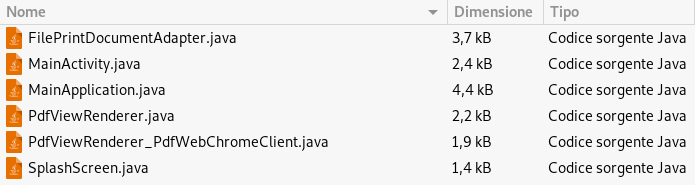
\includegraphics[width=.9\textwidth]{reverse/sources}}
	\caption{File JAVA ottenuti dall'apk.}
	\label{fig:sources}
\end{figure}

\subsection{Descrizione della vulnerabilità}

Un'applicazione Android viene definita vulnerabile al \emph{reverse engineering} quando un attaccante è in grado di effettuare una delle seguenti operazioni\cite{reverse}:
\begin{itemize}
	\item Risalire al codice sorgente originale partendo dai file binari
	\item Ottenere il contenuto di una \emph{string table} binaria
	\item Eseguire analisi \emph{cross functional}
\end{itemize}

L'offuscamento del codice è quel processo tramite il quale viene modificato l'eseguibile in maniera tale da non essere più facilmente interpretabile dall'attaccante pur mantenendo le stesse funzionalità dell'originale.

Pur nella considerazione che con adeguati sforzi ed abbastanza tempo si può rivelare il codice sorgente di pressoché qualunque applicazione Android tramite  reverse engineering, l'assenza di processi di offuscamento rende l'operazione particolarmente banale. Tale mancanza ha permesso la decompilazione dell'apk originale alla maggior parte degli strumenti a mia disposizione (figura \ref{fig:source} e \ref{fig:sources}).

Le possibili varianti di offuscamento sono tantissime. A titolo di esempio si citano:

\begin{itemize}
	\item Ridenominazione di variabili o funzioni (figura \ref{fig:reverse1})
	\item Crittazione delle stringhe (figura \ref{fig:reverse2})
	\item Inserimento di codice inutilizzato
	\item Modifica del flusso di esecuzione
\end{itemize}

\begin{figure}[h]
	\centering
	\subfloat[]{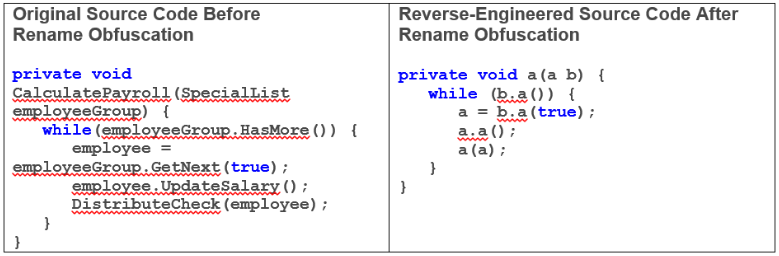
\includegraphics[width=.9\textwidth]{reverse/reverse1}\label{fig:reverse1}} \\
	\subfloat[]{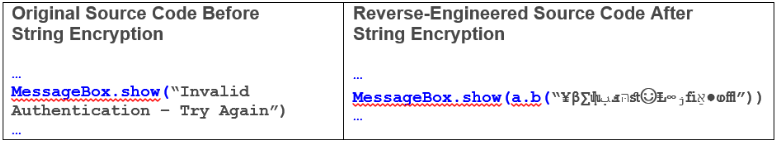
\includegraphics[width=.9\textwidth]{reverse/reverse2}\label{fig:reverse2}}
	\caption{Esempi di offuscamento del codice.}
	\label{fig:obfuscation}
\end{figure}

\subsection{Contromisure}
È consigliabile utilizzare una o più tecniche di offuscamento del codice. È importante notare che l'utilizzo di alcune di queste tecniche può comportare un calo delle prestazioni a causa delle operazioni di decodifica.

Esistono strumenti specifici in grado di applicare automaticamente le tecniche principali lasciando all'utente l'unico compito di trovare il giusto compromesso tra offuscamento e prestazioni.

\section{Possibile backup}

\begin{figure}[h]
	\centering 
	\fbox{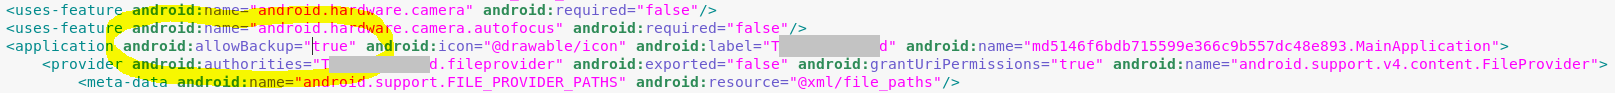
\includegraphics[width=.9\textwidth]{backup/backup}}
	\caption{Estratto dal manifest.}
	\label{fig:backup}
\end{figure}

\subsection{Descrizione della vulnerabilità}

Come visibile in figura \ref{fig:backup}, è presente nel manifest l'opzione:
\begin{center}
	\emph{android:allowBackup="true"}
\end{center}

Con questa opzione attiva è possibile effettuare un backup completo dell'applicazione che, con i privilegi di root, può comprendere anche le \emph{shared preference}, tutti i file, i database e l'apk stesso.
\begin{figure}[h]
	\centering 
	\fbox{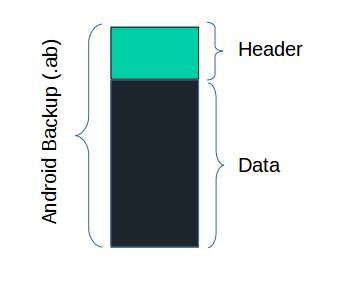
\includegraphics[width=.5\textwidth]{backup/exploit}}
	\caption{Formato backup app Android.}
	\label{fig:structure}
\end{figure}

Analizzando poi la struttura di un backup Android (figura \ref{fig:structure}) e sapendo che nell'intestazione non è presente alcun riferimento ai dati contenuti nel backup, diventa chiara l'esposizione ad un attacco che permette di modificare i dati contenuti nel backup e reinserire la nuova versione modificata nel dispositivo. Tale attacco può essere riassunto in questi passaggi:

\begin{itemize}
	\item Ottenere il backup (ad esempio tramite adb)
	\item Separare i dati dall'intestazione del backup
	\item Modificare a piacimento i dati dell'applicazione
	\item Reimpacchettare i nuovi dati
	\item Recuperare l'intestazione dal backup originale
	\item Anteporre l'intestazione ai nuovi dati
	\item Ripristinare il backup  con i nuovi dati nel dispositivo (esso verrà accettato senza alcuna richiesta dato che verrà riconosciuta l'intestazione dell'applicazione originale)
\end{itemize}

\subsection{Contromisure}

Evitare questo tipo di attacco è molto semplice; se non è strettamente necessario dover effettuare backup dell'applicazione, è sufficiente settare l'opzione \emph{android:allowBackup} a false e sarà il sistema operativo stesso a non permettere tale operazione.

\section{Attività di logging}

\begin{figure}[h]
	\centering 
	\fbox{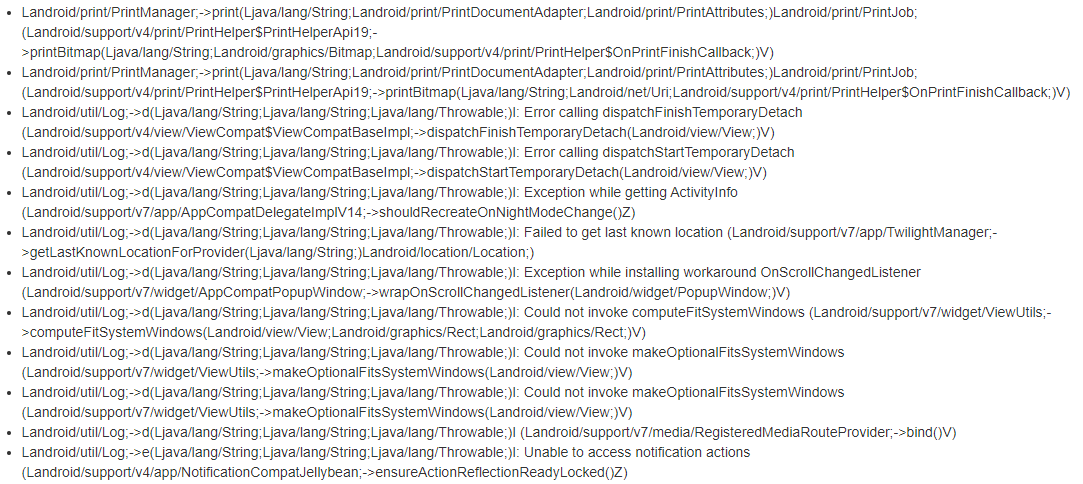
\includegraphics[width=.9\textwidth]{log}}
	\caption{Alcune funzioni che loggano informazioni.}
	\label{fig:log}
\end{figure}

\subsection{Descrizione della vulnerabilità}

Nell'applicazione sono presenti $454$ chiamate a funzioni di log (figura \ref{fig:log}). Alcune di queste potrebbero svelare informazioni riservate o utili all'attaccante.

Analizzando i log non sembra essere presente un rilascio di informazioni utili ma, data la quantità delle funzioni di log presenti, non è stato possibile controllarle tutte approfonditamente. Un attaccante con abbastanza tempo a disposizione potrebbe analizzare completamente i log generati ed ottenere informazioni interessanti.

\subsection{Contromisure}
In questo caso, la pratica migliore è quella di cercare di loggare il minor numero di informazioni possibile; è quindi consigliabile controllare l'effettiva necessità di tutte le funzioni di log presenti rimuovendo eventualmente quelle non necessarie.

\section{Uso di librerie esterne}

\begin{figure}[h]
	\centering 
	\fbox{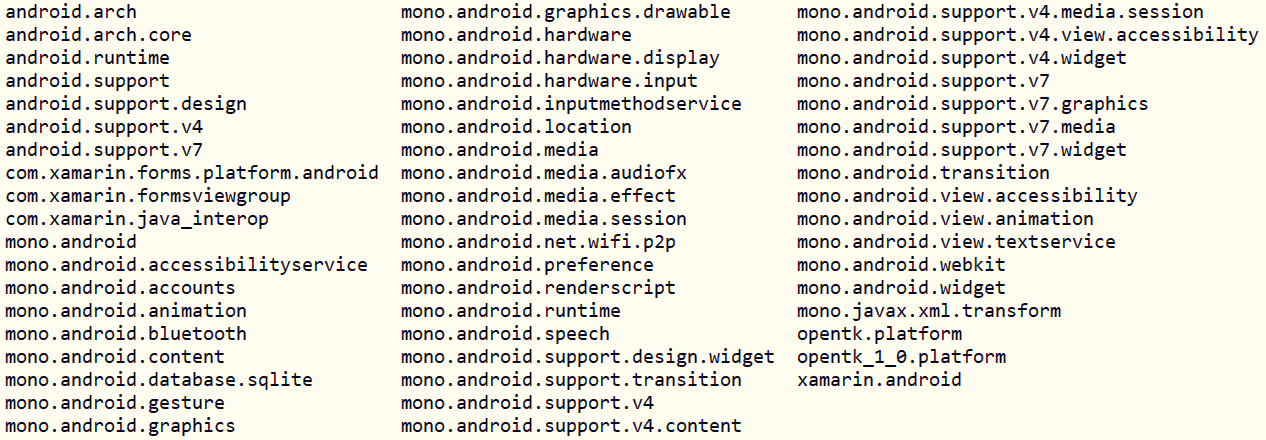
\includegraphics[width=.9\textwidth]{librerie}}
	\caption{Librerie esterne utilizzate.}
	\label{fig:librerie}
\end{figure}

\subsection{Descrizione della vulnerabilità}

All'interno dell'applicazione sono state rilevate un gran numero di librerie esterne (figura \ref{fig:librerie}). Molti strumenti automatici importano automaticamente librerie che possono anche non essere mai utilizzate dallo sviluppatore. Al contrario, l'utilizzo di alcune librerie accelera il processo di sviluppo ma può portare a due tipi di effetti indesiderati:

\begin{itemize}
	\item Una libreria può contenere una vulnerabilità che può rendere vulnerabile l'intera applicazione.
	\item Una libreria può utilizzare una licenza (ad esempio la LGPL$3$) che richiede al creatore dell'applicazione di fornire agli utilizzatori l'accesso al codice sorgente dell'intera applicazione che ne fa uso.
\end{itemize}

\subsection{Contromisure}
Per i motivi esposti sopra, occorre sempre utilizzare il minor numero possibile di librerie esterne, controllando per ognuna la licenza e la presenza di vulnerabilità note.

\section{Permessi pericolosi}

\begin{figure}[h]
	\centering 
	\fbox{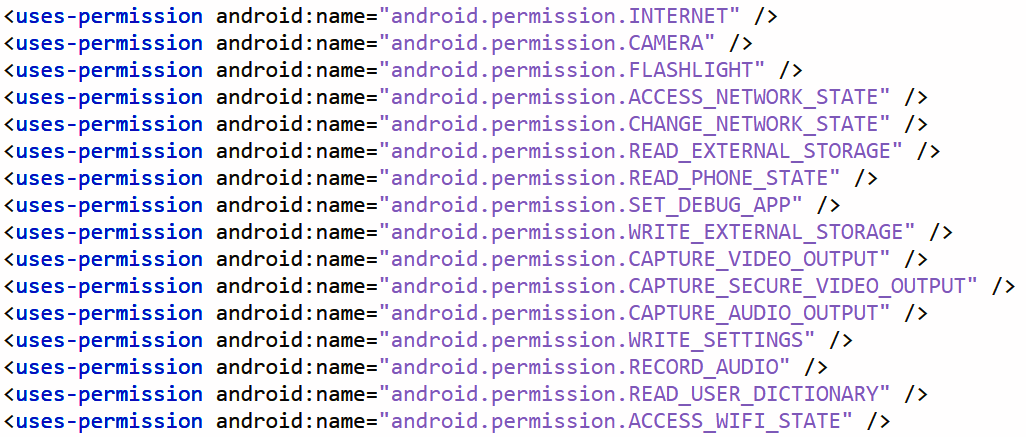
\includegraphics[width=.9\textwidth]{permessi}}
	\caption{Permessi richiesti dall'applicazione.}
	\label{fig:permessi}
\end{figure}

\subsection{Descrizione della vulnerabilità}

Estraendo dal manifest i permessi richiesti dall'applicazione (figura \ref{fig:permessi}) se ne notano alcuni il cui utilizzo può risultare molto pericoloso. 

L'accoppiata \emph{READ EXTERNAL STORAGE} e \emph{WRITE EXTERNAL STORAGE} in particolare, permette all'applicazione l'accesso (in lettura e scrittura) alla memoria esterna del dispositivo. Tale memoria non è protetta dal sistema di isolamento di Android e qualunque file lì presente può essere letto$/$scritto da qualunque applicazione possegga il relativo permesso. Se un attaccante riuscisse a prendere possesso dell'applicazione, potrebbe dunque leggere e scrivere qualunque file, di qualunque applicazione, presente nella memoria esterna.

Da un'analisi dell'applicazione è stato rilevato che la memoria esterna non viene mai utilizzata e quindi la dichiarazione di tali permessi è completamente inutile.

\subsection{Contromisure}
Come precedentemente detto, è fondamentale richiedere il minor numero di permessi possibili, solo quelli strettamente necessari al funzionamento dell'applicazione. Aggiungere permessi inutilizzati ha come unico risultato l'esposizione ad attacchi o utilizzi non previsti (anche illeciti) della stessa.

In questo caso occorre controllare l'effettivo utilizzo e la necessità di ogni singolo permesso richiesto, rimuovendo eventualmente quelli inutilizzati.

\section{Mancata implementazione pinning SSL}

\subsection{Descrizione della vulnerabilità}
Il \emph{pinning} di un certificato è l'associazione del server di backend con uno specifico certificato X.$509$ o una chiave pubblica. Una volta inserito tale certificato/chiave nell'applicazione tramite \emph{hardcoding} o alla prima connessione, si può essere ragionevolmente sicuri che l'applicazione si connetta solamente al server conosciuto evitando possibili attacchi \ac{MITM}.

Il pinning del certificato alla prima connessione dell'applicazione con il server non fornisce comunque una protezione completa se effettuata in un ambiente non controllato. L'attaccante potrebbe comunque intercettare la prima connessione, fornire il proprio certificato che a questo punto verrebbe riconosciuto come legittimo. 

L'implementazione più sicura del pinning dei certificati sarebbe quella dell'hardcoding all'interno dell'applicazione ma questa soluzione crea problemi nel caso di modifiche successive del certificato (scadenza, revoca, ecc...). Per questo motivo, al posto del certificato, si tende ad effettuare il pinning della chiave pubblica del server che dovrebbe avere una durata più estesa.

\subsection{Contromisure}

\begin{figure}[h]
	\centering 
	\fbox{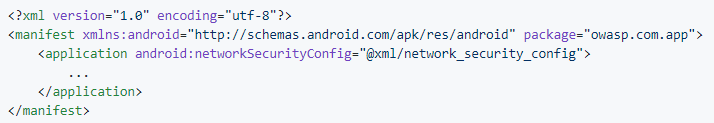
\includegraphics[width=.9\textwidth]{pinning/manifest}}
	\caption{Modifica al manifest.}
	\label{fig:pinningManifest}
\end{figure}

Dall'analisi del codice sorgente dell'applicazione è emersa l'assenza di questo sistema di protezione. Android (dalla versione $7.0$ in poi) fornisce il \emph{Network Security Configuration}, un sistema che permette di impostare una connessione sicura senza modificare il codice sorgente. Le uniche modifiche da effettuare (dopo aver ottenuto un certificato) sono: 
	\begin{itemize}
		\item Aggiungere al manifest la dichiarazione di un file di configurazione di \emph{network security}(figura \ref{fig:pinningManifest}).
		\item La creazione di un file di configurazione (figura \ref{fig:pinningFile}) nel quale inserire un pool di chiavi ritenute affidabili per connettersi al server.
	\end{itemize}

\begin{figure}[h]
	\centering 
	\fbox{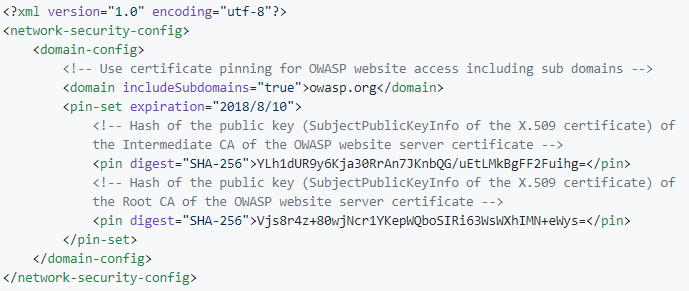
\includegraphics[width=.9\textwidth]{pinning/file}}
	\caption{Modifica al manifest.}
	\label{fig:pinningFile}
\end{figure}

\section{Connessioni non sicure}

\subsection{Descrizione della vulnerabilità}
Le analisi statiche dell'applicazione hanno rilevato $540$ possibili connessioni \ac{HTTP}. Le connessioni \ac{HTTP} sono intrinsecamente insicure in quanto non cifrate in alcun modo. Il traffico in chiaro può quindi essere intercettato e compreso dall'attaccante senza particolari sforzi.

L'analisi manuale del codice ha trasformato questa rilevazione in un falso positivo dato che gli \ac{URL} rilevati sono semplicemente gli schemi dei vari file \ac{XML} (figura \ref{fig:schema}).

\begin{figure}[h]
	\centering 
	\fbox{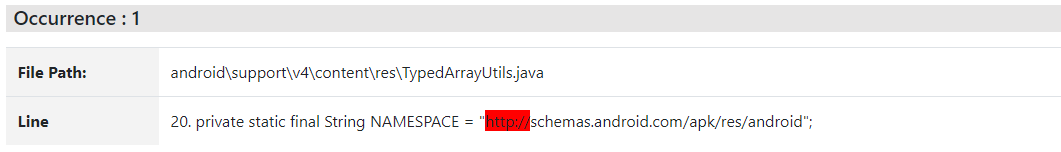
\includegraphics[width=.9\textwidth]{http}}
	\caption{XML schema.}
	\label{fig:schema}
\end{figure}

\subsection{Contromisure}
In generale, occorre sempre utilizzare connessioni \ac{HTTPS} al posto delle connessioni \ac{HTTP}, ma in questo caso non c'è bisogno di alcuna contromisura in quanto non si tratta di vere connessioni.

\section{Possibile screenshot}

\begin{figure}[h]
	\centering 
	\fbox{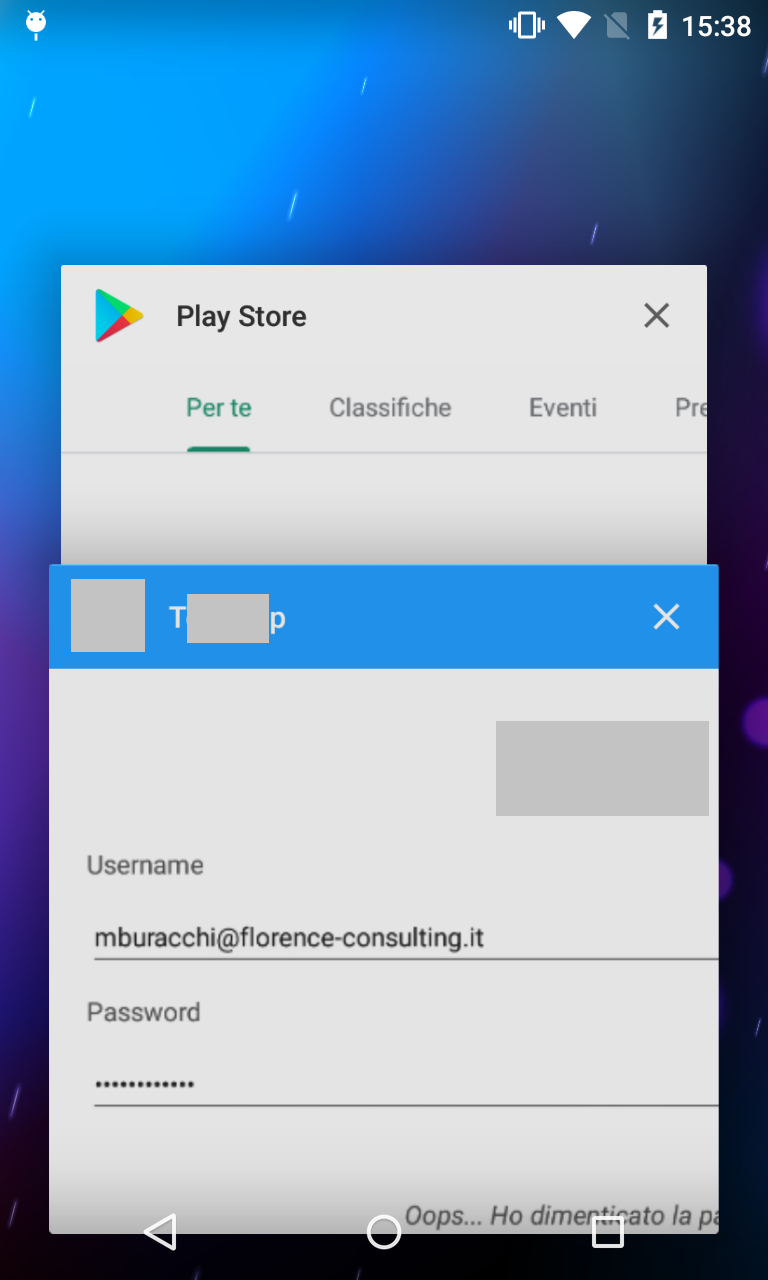
\includegraphics[width=.45\textwidth]{screen/background}}
	\caption{Background screenshot.}
	\label{fig:background}
\end{figure}

\subsection{Descrizione della vulnerabilità}
L'applicazione permette il salvataggio di screenshot. Tale pratica è spesso sconsigliata per due motivi:
\begin{itemize}
	\item Un'applicazione malevola potrebbe effettuare screenshot quando sono presenti dati sensibili sullo schermo (elenco clienti, utenti o transazioni) per ottenere informazioni altrimenti inaccessibili. Gli screenshot sono salvati nella memoria pubblica e possono essere recuperati da qualunque altra applicazione presente sul dispositivo.
	\item Ogni volta che l'applicazione viene messa in background, il sistema operativo effettua uno screenshot per riproporre l'ultima schermata al ritorno in foreground. Tale screenshot è visibile anche nell'elenco delle applicazioni in background (figura \ref{fig:background}).
\end{itemize}

\subsection{Contromisure}
È consigliabile bloccare la possibilità di effettuare screenshot dell'applicazione se non strettamente necessario. Per raggiungere questo obiettivo è sufficiente utilizzare l'opzione \emph{FLAG SECURE} nel metodo \emph{onCreate()} dell'activity che si vuole proteggere (figura \ref{fig:screen}).

\begin{figure}[h]
	\centering 
	\fbox{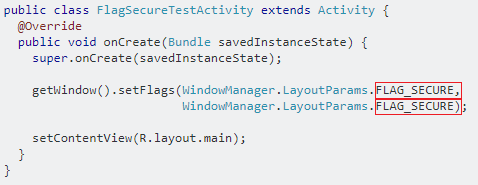
\includegraphics[width=.9\textwidth]{screen/flag}}
	\caption{Esempio di blocco degli screen.}
	\label{fig:screen}
\end{figure}

\section{Activity esportata}

\subsection{Descrizione della vulnerabilità}
L'applicazione esporta una activity. L'esportazione di una activity permette la sua invocazione da parte di un'altra applicazione o del sistema. Esportazioni non necessarie incrementano la superficie d'attacco a disposizione dell'attaccante. Fortunatamente l'unica activity esportata è quella necessaria per l'esecuzione dell'applicazione e quindi non rappresenta un problema. 

\subsection{Contromisure}
Nessuna contromisura necessaria.

\section{Non rileva emulatori$/$debuggers$/$root}

\subsection{Descrizione della vulnerabilità}
Al momento dell'installazione non viene controllato se l'ambiente in cui si eseguirà l'applicazione è sicuro. Eseguire in modalità particolari (ambienti di emulazione, ambienti di debug o dispositivi con permessi di root) un'applicazione che possiede informazioni sensibili, è sempre non sicuro. È quindi buona pratica effettuare dei controlli in merito. 

Nel caso ci trovassimo in un ambiente anomalo, non dovremmo permettere l'installazione dell'applicazione o quantomeno avvertire l'utente del rischio che si corre. 

\subsection{Contromisure}
Purtroppo non esiste una singola procedura per effettuare queste verifiche ma occorre implementare controlli multipli. Tra i più comuni troviamo i seguenti:
\begin{itemize}
	\item Controllare la presenza di alcuni file o binari abitualmente presenti in ambienti con privilegi di root sbloccati (superuser.apk, daemonsu, su, ecc...).
	\item Controllare la presenza del comando \emph{su} nel \emph{PATH}.
	\item Controllare a runtime la presenza di processi attivi riconducibili ad ambienti non sicuri.
	\item Tramite il gestore pacchetti di Android, verificare la presenza di applicazioni che operano in ambienti non sicuri.
	\item Controllare la modalità di montaggio delle partizioni del sistema. Quando si sbloccano i privilegi di root, esse vengono montate in modalità lettura$/$scrittura mentre normalmente sono montate in sola lettura.
	\item Controllare di non essere su una ROM custom. 
\end{itemize} 